Při návrhu aktivní zátěže, začneme návrhem rozměrů tranzistorů.
Délku kanálu \(L\) zvolíme opět \(L = 2 [\mu m]\) a napětí \(U_{TH} = 0.2 [V]\), šířku kanálu \(W\) pak určíme jako:

\begin{center}
    \large
    \(
        W_{M2} = W_{M3} = L \cdot \frac{2 \cdot I_d}{KP \cdot U_{OV}^2} = 2\mu \cdot \frac{2 \cdot 10\mu}{200\mu 0.2^2} = 5 [\mu m]
    \)
\end{center}

Následně určíme odpor nastavující proud tranzistorem \(M_3\) jako:

\begin{center}
    \large
    \(
        R_{1} = \frac{U_{CC} - (U_{TH} + U_{OV})}{I_D} = \frac{1.8-(0.4+0.2)}{10\mu} = 120 [k\Omega] 
    \)
\end{center}

\vspace{10mm}
\begin{figure}[h!]
    \centering
    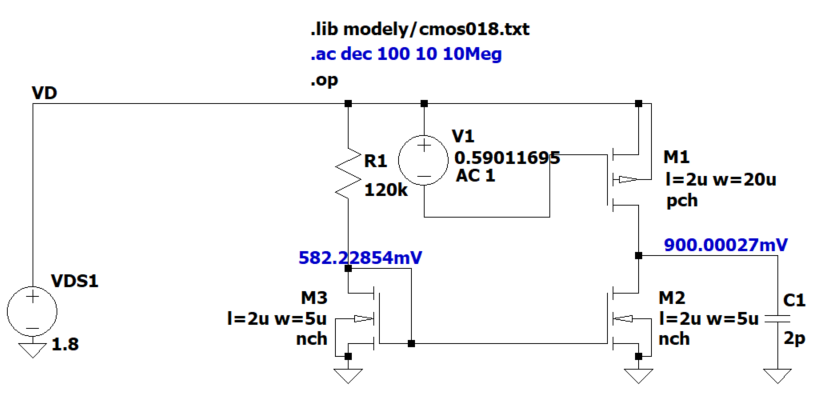
\includegraphics[width=0.8\textwidth]{text/img/Akt-sch.png}
    \caption{\label{fig:Akt-sch} Schéma zesilovače s aktivní zátěží}
\end{figure}

\vspace{10mm}
\begin{figure}[h!]
    \centering
    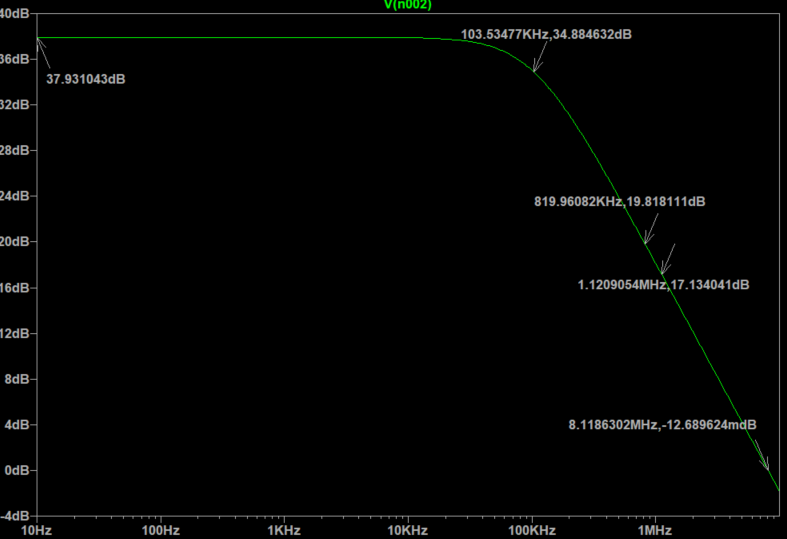
\includegraphics[width=0.7\textwidth]{text/img/Akt-AC-graf.png}
    \caption{\label{fig:Akt-AC} {\bf .AC} analýza zesilovače s aktivní zátěží}
\end{figure}

Zesílení s aktivní zátěží vychází o \(19 [dB]\) vyšší než v případě s odporovou zátěží.
Pokles o \(3 [dB]\) nastává mnohem dříve místo \(824 [kHz]\) už při \(104 [kHz]\).
Naproti tomu i při frekvenci \(824 [kHz]\) má zesilovač vyšší zesílení než případ z odporovou zátěží a ke stejnému zesílení, tedy \(17 [dB]\) dochází až u frekvence \(1.12 [MHz]\).
Zesilovač s aktivní zátěží má ale strmější pokles, protože přestává zesilovat na frekvenci \(GBW = 8.12 [MHz]\), zatím co odporová varianta zesiluje až do \(GBW = 8.43 [MHz]\).

\vspace{10mm}
\begin{figure}[h!]
    \centering
    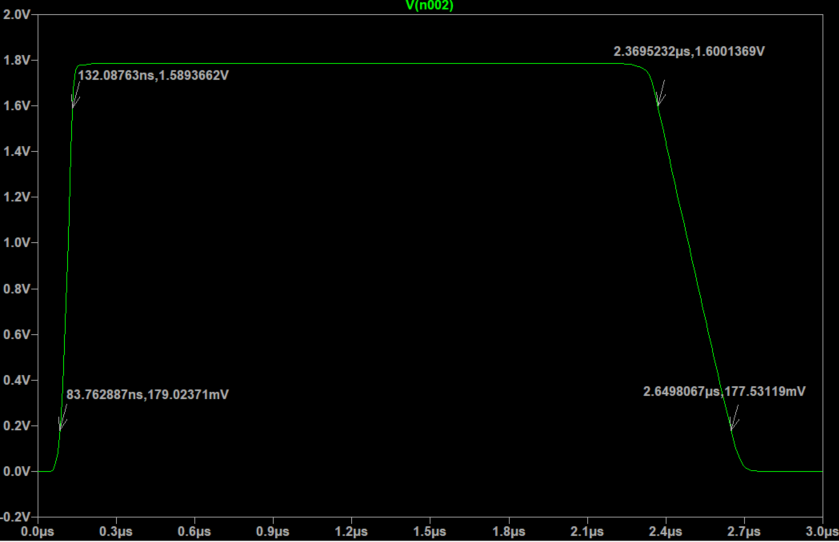
\includegraphics[width=0.7\textwidth]{text/img/Akt-trans-graf.png}
    \caption{\label{fig:res-SR} {\bf .trans} analýza s vyznačenými body pro určení SR}
\end{figure}

Z průběhu \ref{fig:res-SR} určíme SR jako:
\begin{center}
    \Large
    \(
        SR_{rise} = \frac{\Delta U}{\Delta t} = \frac{U_2 - U_1}{t_2 - t_1} = \frac{1.589 - 0.179}{132n - 87n} = 31.3 [V/\mu s]
    \)

    \(
        SR_{fell} = \frac{\Delta U}{\Delta t} = \frac{U_1 - U_2}{t_2 - t_1} = \frac{1.6 - 0.178}{2650n - 2367n} = 5 [V/\mu s]
    \)
\end{center}

Zde je vidět že sestupná hrana už zadání přesně splňuje.
